\chapter{Compilación del \emph{kernel}}

\section{Introducción}

La compilación se refiere al proceso de traducción de un lenguaje de alto nivel
a otro funcionalmente equivalente, expresado en lenguaje ensamblador de una
arquitectura específica\cite{compilacion}. Durante este capítulo se explica la
técnica para crear una toolchain que genere binarios para la plataforma PPC405.


\section{El proceso de compilación}

El proceso de compilación es el proceso por el cual se traducen las
instrucciones escritas en un determinado lenguaje de programación a lenguaje
máquina. Además de un traductor, se pueden necesitar otros programas para crear
un programa objeto ejecutable. Un programa fuente se puede dividir en módulos
almacenados en archivos distintos. La tarea de reunir el programa fuente a
menudo se confía a un programa distinto, llamado preprocesador. El preprocesador
también puede expandir abreviaturas, llamadas a macros, a proposiciones del
lenguaje fuente.

\begin{figure}[ht]
 \centering
 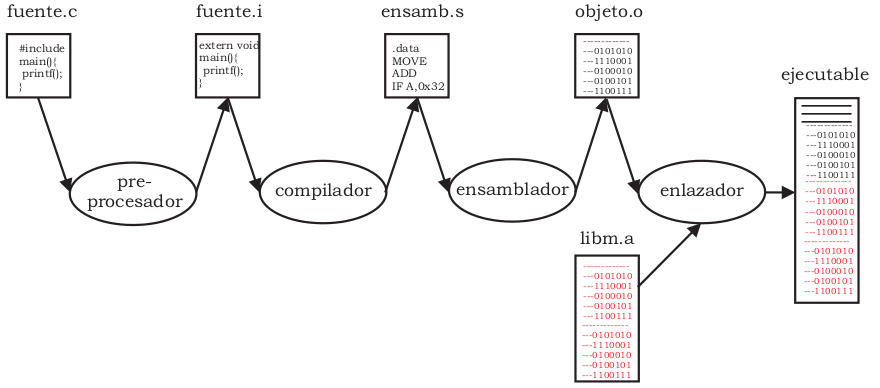
\includegraphics[scale=.45]{./figuras/compilacion.png}
 % capas.png: 607x522 pixel, 72dpi, 21.41x18.41 cm, bb=0 0 607 522
 \caption{El proceso de compilación}
 \label{El proceso de compilación}
\end{figure}

Este proceso se compone internamente de varias etapas mostradas a continuación:

\begin{itemize}
 \item Análisis léxico, se encarga de la reducción del texto del programa en
  \emph{tokens}:
    \begin{itemize}
      \item identificadores
      \item separadores operadores
      \item constantes
    \end{itemize}

  \item Análisis sintáctico, se encarga del análisis de símbolos para
  reconocer la estructura de programa:
  \begin{itemize}
   \item indentificador = expresión
   \item indentificador + constante
  \end{itemize}
  
  \item Análisis semántico, realiza la asociación de identificadores con zonas
  de memoria y la asociación de tipos de datos.

  \item Generación de código, Asocia las sentencias con secuencias de
  instrucciones.
  
  \item Optimización de código, consiste en mejorar el código intermedio, de
  modo que resulte un código máquina más rápido de ejecutar.

\end{itemize}

\section{Compilación cruzada}

Si un compilador es capaz de compilar un programa para otra arquitectura en la
cual se está ejecutando, se dice que es un compilador cruzado. En este proceso
se identifica al equipo que realiza la compilación mediante el término
\emph{Host} o Huesped y al dispositivo que ejecuta el software, como sistema
\emph{Target} u Objetivo\cite{building}.

\subsection{Sistema huesped}

La implementación de un entorno de compilación cruzada nos brinda la
posibilidad de aprovechar los recursos que disponemos en una PC. Esta tarea se
ha llevado a cabo sobre una PC de escritorio con las siguientes características:

\begin{itemize}
 \item 2 Procesadores Intel(R) Core(TM) 2 Duo 3.16GHz
 \item Memoria 1.9 GiB
 \item Sistema Operativo Debian GNU/Linux 6.0.5 (squeeze)
 \item Kernel Linux 2.6.32-5-amd64
\end{itemize}


\subsection{Sistema objetivo}

El sistema objetivo es la tarjeta de desarrollo XUPV2, dentro de ella se
cuenta con un FPGA Xilinx Virtex-II Pro 50 con las siguientes características:

  \begin{itemize}
  \item FPGA Virtex-2 Pro XC2VP30  con 30,816 celdas lógicas, 136 18-bit
multiplicadores,
  2,448Kb bloques de RAM y 2 Procesadores PowerPC.
  \item DDR SDRAM DIMM de hasta  2Gbytes de RAM
  \item Puerto Ethernet 10/100
  \item Puerto USB2 
  \item Lector de tarjetas Compact Flash
  \item Puerto de video XSGA
  \item Audio Codec
  \item Puertos SATA, S/2 y RS-232
  \end{itemize}
   
\begin{figure}[ht]
 \centering
 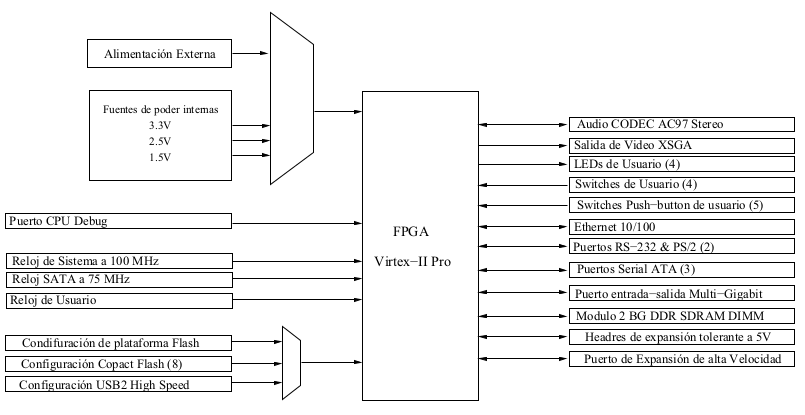
\includegraphics[scale=.50]{./figuras/virtex.png}
 % capas.png: 607x522 pixel, 72dpi, 21.41x18.41 cm, bb=0 0 607 522
 \caption{Diagrama a bloques de la tarjeta Virtex-II Pro 50}
 \label{Diagrama a bloques de la tarjeta Virtex-II Pro 50}
\end{figure}

Estas características proporcionan un gran número de posibilidades para
el desarrollo de aplicaciones y, puesto que existen hoy en día herramientas de
software que ayudan a la programación, compilación, sıntesis, simulación y
depuración tanto de hardware como de software, se obtiene una alta flexibilidad
de desarrollo, permitiendo a los usuarios centrarse en el diseño y tomando la
responsabilidad de dicho diseño para obtener el máximo provecho de los
recursos\cite{alvarado}.



\subsection{GNU \emph{toolchain}}

GNU toolchain es un término que agrupa a una serie de proyectos que contienen
las herramientas de programación producidas por el proyecto GNU. Estos proyectos
forman un sistema integrado que es usado para programar tanto aplicaciones como
sistemas operativos.

El GNU toolchain es un componente vital en el desarrollo del núcleo Linux, el
desarrollo del BSD y software para sistemas empotrados.

Cualquier compilador requere librerías de soporte (como
\emph{libc}\footnote{\emph{libc}, es una recopilación de ficheros cabecera y
bibliotecas con rutinas, estandarizadas por un comité de la Organización
Internacional para la Estandarización (ISO), }) además de bianrios
(ensambladores y \emph{linkers}), una \emph{toolchain} requiere estos mismos
componentes también, una \emph{toolchain} tiene los componentes enlistados a
continuación:
\begin{itemize}
 \item \emph{Binutils}, es un conjunto de programas necesarios para el enlace,
 ensable y compilación.
 \item Compilador GNU, compilador básico de lenguaje C, usado para obtener un
código objeto.
 \item Librerías C GNU, esta librería implementa llamadas al sistema, cualquier
aplicación desarrollada necesita ser ligada a esta librería base.
\end{itemize}

\section{Construyendo una \emph{toolchain}}

Los pasos para construir una \emph{toolchain} se citan a continuación:
\begin{enumerate}
 \item Decidir el sistema objetivo.
 \item Decidir versiones de \emph{kernel/gcc/glibc/binutlis}.
 \item Compilar \emph{binutlis}.
 \item Obtener los \emph{kernel headers} para la plataforma objetivo.
 \item Compilar una versión minima de \emph{gcc}.
 \item Construir \emph{glibc}.
 \item Recompilar \emph{gcc}.
\end{enumerate}

\section{Fuentes del \emph{kernel}}

El \emph{kernel} de Linux puede obtenerse desde muchos repositorios, sin
embargo la fuente principal para descarga se encuentra disponible en
\emph{http://www.kernel.org/} en donde se puede descargar la versión actual
disponible así como también versiones anteriores.

\subsection{linux-xlnx}

\emph{linux-xlnx} es una rama del \emph{kernel} mantenida por la empresa
Xilinx, la cual tiene actualizados una serie de parches y ofrece soporte para
una amplia gama de periféricos presentes en sus tarjetas de desarrollo.

Para obtener este \emph{kernel} se usa el siguiente comando:

\begin{verbatim}
 Proyecto@debian$ git clone git://git.xilinx.com/linux-2.6-xlnx.git
\end{verbatim}



\section{Configuración del \emph{kernel}}


El \emph{kernel} de Linux debe de ser compilado con la ayuda de una
\emph{toolchain} que nos permita alcanzar la arquitectura objetivo
(\emph{PowerPC 405}).

La \emph{toolchain} usada en este proyecto para compilar el \emph{kernel} esta
descrita en el protecto terminal \emph{``Plataforma para la ejecución paralela
en un sistema embebido basado en FPGA''}\cite{Beto}, para cargar las variables
de entorno necesarias para el uso de la \emph{toolchain} se ejecuta el siguiente
\emph{script}:


\begin{verbatim}
 Proyecto@debian$ source
/home/Proyecto/Crosstool/powerpc-405-linux-uclibc/loadembenv.sh
\end{verbatim}


\lstinputlisting[caption=Archivo loadembenv.sh,language=sh]
{./code/loadembenv.sh}


El archivo ``.config'' se usa para controlar las partes del \emph{kernel} que
serán incluidas, se debe de ser muy cuidadoso con la configuración del
\emph{kernel}, si se selecciona algún componente de manera errónea la
compilación puede fallar.

No es  recomendable editar el archivo ``.config'' directamente, existen
programas que ayudan a la configuración de este archivo como
\emph{makmenuconfig} y \emph{make xconfig}, el archivo ``.config''
configurado se muestra en el \emph{Apéndice B}.

Una vez que se configura el \emph{kernel}, se procede a la compilación con el
siguiente comando:
\begin{verbatim}
  Proyecto@debian$ make simpleImage.virtex405-nombre_del_proyecto
\end{verbatim}


\section{system.ace}


\emph{System Advanced Configuration Environment} (System ACE) es una tecnología
que proporciona un ahorro sustancial en el desarrollo y el costo por bit de
almacenamiento.

\begin{figure}[ht]
 \centering
 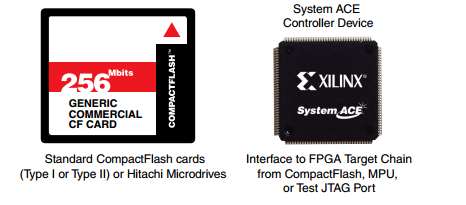
\includegraphics[scale=.70]{./figuras/SystemACE.png}
 % capas.png: 607x522 pixel, 72dpi, 21.41x18.41 cm, bb=0 0 607 522
 \caption{SystemACE}
 \label{SystemACE}
\end{figure}

La tarjeta de desarrollo \emph{XUPV2P} puede hacer la carga por
\emph{system.ace} de los archivos ELF (\emph{Executable and Linkable Format}),
el archivo ``simpleImage.virtex405-micheangeloEXT2.elf'' generado en la
compilación del \emph{kernel} se encuentra en la ruta
\emph``/arch/powerpc/boot/'' del directorio del \emph{kernel}.

Para generar el ``systme.ace'' se utiliza el siguiente archivo de configuración:

\lstinputlisting[caption=Archivo xupGenaceEXT2.opt,language=C]{
./code/xupGenaceEXT2.opt}

Y se procede con el comando:
\begin{verbatim}
 Proyecto@debian$ xmd -tcl genace.tcl -opt xupGenaceEXT2.opt
\end{verbatim}

El comando anterior genera el archivo ``system.ace'' el cual contiene la
configuración del \emph{kernel} que funcionará en la tarjeta, este archivo
junto con la configuración obtenida al diseñar el \emph{hardware} en el archivo
``xilinx.dts'' determinará la forma de arranque de nuestro sistema embebido.






